\documentclass[tikz,multi=tikzpicture,border=7pt]{standalone}
\usepackage{ctex}
\usepackage{amsmath,amssymb,bm}
\usetikzlibrary{arrows.meta,calc,decorations.pathmorphing,patterns,positioning,angles,quotes,3d}
\tikzset{
  vec/.style={-{Latex[length=2.6mm]},very thick,blue!72!black},
  force/.style={-{Latex[length=2.6mm]},very thick,red!72!black},
  guide/.style={gray!65,dashed},
  body/.style={draw,very thick,fill=blue!8},
  mass/.style={draw,very thick,fill=orange!45,rounded corners=1pt},
  dim/.style={<->,>=Latex,thin},
  ray/.style={-{Latex[length=2.3mm]},very thick,orange!82!black},
  curve/.style={very thick,blue!70!black}
}
\tikzset{vec/.style={-{Latex[length=2.4mm]},very thick,blue!70!black},force/.style={-{Latex[length=2.4mm]},very thick,red!70!black},impulse/.style={force},ray/.style={-{Latex[length=2.2mm]},thick,orange!80!black},wave/.style={blue!70!black,thick},body/.style={draw,very thick,fill=blue!7},guide/.style={gray!65,dashed},dim/.style={<->,>=Latex,thin},resistor/.style={decorate,decoration={zigzag,segment length=4pt,amplitude=2pt},thick}}
\begin{document}

% 1 question-01
\begin{tikzpicture}[x=1cm,y=1cm,font=\small]

\fill[blue!8](0,0)--(4.3,0)--(3.04,3.04)--cycle;\draw[very thick](0,0)--(4.8,0)node[right]{$B$};\draw[very thick](0,0)--(3.4,3.4)node[above]{$A$};
\fill(0,0)circle(2pt)node[below left]{$O$};\fill(2.828,2.828)circle(2pt)node[above left]{$D$};\fill(4,0)circle(2pt)node[above]{$C$};\fill(4,-2)circle(2pt)node[below]{$H$};\draw[guide](4,0)--(4,-2);
\draw[dim](0,-.5)--(4,-.5)node[midway,below]{$l=1$ km};\draw[dim](4.6,0)--(4.6,-2)node[midway,right]{$h=.5$ km};\draw(.8,0)arc(0:45:.8)node[right]{$\alpha=45^\circ$};\node[above left]at(1.4,1.4){$x=1$ km};\node at(2.8,1){海水：$v/n$};\node at(1.5,-1.3){陆地：$v$};
\end{tikzpicture}

% 2 solution-01
\begin{tikzpicture}[x=1cm,y=1cm,font=\small]
\begin{scope}[shift={(-3.5,0)}]
\draw[very thick](0,0)--(4.4,0);\draw[very thick](0,0)--(3.2,3.2);\draw[vec] plot coordinates {(4.00000,-2.00000) (3.30131,0.00000)};
\draw[vec,green!50!black] plot coordinates {(3.30131,0.00000) (2.82843,2.82843)};
\fill(4,-2)circle(2pt)node[below]{$H$};\fill(3.30131,0)circle(2pt)node[below right]{$E$};\fill(2.828,2.828)circle(2pt)node[above left]{$D$};\draw[guide](3.30131,-.7)--(3.30131,1);\node[align=center]at(2,-3){$OE=.82533$ km\\$t_2=1963.475$ s};\end{scope}
\begin{scope}[shift={(3.5,0)}]
\draw[very thick](0,0)--(4.4,0);\draw[very thick](0,0)--(3.2,3.2);\draw[vec] plot coordinates {(4.00000,-2.00000) (2.79000,0.00000)};
\draw[vec,green!50!black] plot coordinates {(2.79000,0.00000) (2.20040,2.20040)};
\draw[vec] plot coordinates {(2.20040,2.20040) (2.82843,2.82843)};
\fill(4,-2)circle(2pt)node[below]{$H$};\fill(2.79000,0)circle(2pt)node[below right]{$F$};\fill(2.828,2.828)circle(2pt)node[above left]{$D$};\draw[guide](2.79000,-.7)--(2.79000,1);\draw[guide](1.70040,2.70040)--(2.70040,1.70040);\node[left]at(2.20040,2.20040){$G$};\node[align=center]at(2,-3){$OF=.69750$ km，$OG=.77796$ km\\$t_3=1945.438$ s};\end{scope}

\end{tikzpicture}

% 3 question-02
\begin{tikzpicture}[x=1cm,y=1cm,font=\small]
\draw[very thick] plot coordinates {(0.00000,0.00000) (0.04040,-0.33431) (0.08081,-0.64985) (0.12121,-0.94765) (0.16162,-1.22870) (0.20202,-1.49393) (0.24242,-1.74419) (0.28283,-1.98033) (0.32323,-2.20310) (0.36364,-2.41326) (0.40404,-2.61148) (0.44444,-2.79842) (0.48485,-2.97469) (0.52525,-3.14088) (0.56566,-3.29753) (0.60606,-3.44515) (0.64646,-3.58424) (0.68687,-3.71525) (0.72727,-3.83860) (0.76768,-3.95471) (0.80808,-4.06396) (0.84848,-4.16670) (0.88889,-4.26328) (0.92929,-4.35401) (0.96970,-4.43920) (1.01010,-4.51911) (1.05051,-4.59402) (1.09091,-4.66416) (1.13131,-4.72978) (1.17172,-4.79108) (1.21212,-4.84827) (1.25253,-4.90154) (1.29293,-4.95106) (1.33333,-4.99700) (1.37374,-5.03950) (1.41414,-5.07870) (1.45455,-5.11474) (1.49495,-5.14773) (1.53535,-5.17779) (1.57576,-5.20500) (1.61616,-5.22946) (1.65657,-5.25125) (1.69697,-5.27045) (1.73737,-5.28711) (1.77778,-5.30129) (1.81818,-5.31303) (1.85859,-5.32238) (1.89899,-5.32937) (1.93939,-5.33401) (1.97980,-5.33633) (2.02020,-5.33633) (2.06061,-5.33401) (2.10101,-5.32937) (2.14141,-5.32238) (2.18182,-5.31303) (2.22222,-5.30129) (2.26263,-5.28711) (2.30303,-5.27045) (2.34343,-5.25125) (2.38384,-5.22946) (2.42424,-5.20500) (2.46465,-5.17779) (2.50505,-5.14773) (2.54545,-5.11474) (2.58586,-5.07870) (2.62626,-5.03950) (2.66667,-4.99700) (2.70707,-4.95106) (2.74747,-4.90154) (2.78788,-4.84827) (2.82828,-4.79108) (2.86869,-4.72978) (2.90909,-4.66416) (2.94949,-4.59402) (2.98990,-4.51911) (3.03030,-4.43920) (3.07071,-4.35401) (3.11111,-4.26328) (3.15152,-4.16670) (3.19192,-4.06396) (3.23232,-3.95471) (3.27273,-3.83860) (3.31313,-3.71525) (3.35354,-3.58424) (3.39394,-3.44515) (3.43434,-3.29753) (3.47475,-3.14088) (3.51515,-2.97469) (3.55556,-2.79842) (3.59596,-2.61148) (3.63636,-2.41326) (3.67677,-2.20310) (3.71717,-1.98033) (3.75758,-1.74419) (3.79798,-1.49393) (3.83838,-1.22870) (3.87879,-0.94765) (3.91919,-0.64985) (3.95960,-0.33431) (4.00000,0.00000)};

\draw[body](0,0)circle(.15)node[left]{$m$};\draw[body](4,0)circle(.15)node[right]{$m$};\draw[dim](0,.7)--(4,.7)node[midway,above]{$l$};\draw[dim](4.7,0)--(4.7,-5.33662)node[midway,right]{$h$};
\node[align=left,anchor=west]at(5.3,-1.4){重绳长 $3l$，质量 $M$\\初始位置由支承维持\\后续去掉支承，轻绳仍连接两球};
\end{tikzpicture}

% 4 solution-02
\begin{tikzpicture}[x=1cm,y=1cm,font=\small]

\begin{scope}[shift={(-3.8,0)}]\draw[very thick](-1.8,1.3)..controls(-1.6,-.6)and(-.8,-1.2)..(1.2,-1.2);\draw[force](-1.8,1.3)--(-2.3,2.4)node[above]{$F_1$};\draw[force](1.2,-1.2)--(2.4,-1.2)node[right]{$F_2$};\draw[force](-.7,-.1)--(-.7,-1.7)node[below]{$Mg/2$};\node[align=center]at(0,-3){$F_1^2-F_2^2=(Mg/2)^2$\\$F_1-F_2=\lambda gh$};\end{scope}
\begin{scope}[shift={(3.5,0)}]\foreach\y/\lab in{1.7/碰前,0/碰后,-1.7/绷紧后}{\node[left]at(-2.6,\y){\lab};\draw[body](-1,\y)circle(.15);\draw[body](1,\y)circle(.15);}
\draw[vec](1,1.7)--(-.2,1.7)node[above]{$v_0$};\draw[vec](-1,0)--(-2.2,0)node[above]{$v_0$};\draw[vec](-1,-1.7)--(-1.7,-1.7);\draw[vec](1,-1.7)--(.3,-1.7);\node[below]at(0,-2){两球均 $-v_0/2$，$J_R=mv_0/2$};\end{scope}
\end{tikzpicture}

% 5 question-03
\begin{tikzpicture}[x=1cm,y=1cm,font=\small]
\draw[->](-2,0)--(3.4,0)node[right]{$x$};\draw[->](0,-2.4)--(0,2.3)node[above]{$y$};\draw[very thick,blue!70!black] plot coordinates {(-0.00983,-0.00000) (-0.01003,-0.00063) (-0.01019,-0.00129) (-0.01032,-0.00198) (-0.01040,-0.00268) (-0.01044,-0.00341) (-0.01043,-0.00415) (-0.01037,-0.00490) (-0.01027,-0.00567) (-0.01011,-0.00645) (-0.00990,-0.00723) (-0.00963,-0.00802) (-0.00931,-0.00880) (-0.00893,-0.00958) (-0.00850,-0.01035) (-0.00800,-0.01111) (-0.00745,-0.01185) (-0.00684,-0.01257) (-0.00617,-0.01326) (-0.00544,-0.01393) (-0.00465,-0.01456) (-0.00381,-0.01516) (-0.00291,-0.01571) (-0.00195,-0.01622) (-0.00095,-0.01667) (0.00011,-0.01707) (0.00121,-0.01741) (0.00236,-0.01769) (0.00354,-0.01789) (0.00477,-0.01803) (0.00603,-0.01809) (0.00732,-0.01806) (0.00863,-0.01796) (0.00996,-0.01777) (0.01131,-0.01749) (0.01267,-0.01711) (0.01403,-0.01664) (0.01538,-0.01608) (0.01673,-0.01541) (0.01806,-0.01465) (0.01937,-0.01378) (0.02066,-0.01281) (0.02190,-0.01174) (0.02310,-0.01057) (0.02425,-0.00929) (0.02534,-0.00792) (0.02637,-0.00644) (0.02732,-0.00488) (0.02819,-0.00321) (0.02896,-0.00146) (0.02965,0.00037) (0.03022,0.00229) (0.03069,0.00429) (0.03104,0.00635) (0.03126,0.00848) (0.03134,0.01067) (0.03129,0.01290) (0.03110,0.01518) (0.03075,0.01749) (0.03024,0.01983) (0.02958,0.02218) (0.02875,0.02454) (0.02775,0.02689) (0.02658,0.02922) (0.02524,0.03153) (0.02372,0.03380) (0.02202,0.03601) (0.02015,0.03816) (0.01810,0.04023) (0.01587,0.04222) (0.01347,0.04410) (0.01090,0.04586) (0.00817,0.04749) (0.00527,0.04898) (0.00222,0.05032) (-0.00097,0.05148) (-0.00431,0.05246) (-0.00778,0.05325) (-0.01137,0.05383) (-0.01507,0.05419) (-0.01887,0.05432) (-0.02275,0.05420) (-0.02671,0.05384) (-0.03072,0.05321) (-0.03477,0.05231) (-0.03885,0.05113) (-0.04293,0.04966) (-0.04700,0.04790) (-0.05104,0.04584) (-0.05504,0.04348) (-0.05895,0.04082) (-0.06278,0.03785) (-0.06649,0.03457) (-0.07007,0.03099) (-0.07349,0.02710) (-0.07673,0.02291) (-0.07976,0.01843) (-0.08257,0.01367) (-0.08513,0.00862) (-0.08741,0.00331) (-0.08940,-0.00226) (-0.09106,-0.00806) (-0.09239,-0.01410) (-0.09336,-0.02034) (-0.09394,-0.02677) (-0.09412,-0.03336) (-0.09388,-0.04011) (-0.09320,-0.04697) (-0.09207,-0.05393) (-0.09046,-0.06096) (-0.08837,-0.06803) (-0.08577,-0.07510) (-0.08267,-0.08215) (-0.07906,-0.08915) (-0.07492,-0.09605) (-0.07024,-0.10283) (-0.06504,-0.10945) (-0.05931,-0.11586) (-0.05305,-0.12203) (-0.04626,-0.12793) (-0.03895,-0.13350) (-0.03114,-0.13872) (-0.02283,-0.14354) (-0.01404,-0.14793) (-0.00479,-0.15183) (0.00490,-0.15522) (0.01500,-0.15806) (0.02549,-0.16030) (0.03634,-0.16191) (0.04751,-0.16285) (0.05897,-0.16309) (0.07068,-0.16260) (0.08260,-0.16135) (0.09467,-0.15930) (0.10686,-0.15643) (0.11911,-0.15272) (0.13137,-0.14814) (0.14358,-0.14268) (0.15569,-0.13632) (0.16763,-0.12905) (0.17935,-0.12087) (0.19078,-0.11176) (0.20186,-0.10173) (0.21251,-0.09079) (0.22267,-0.07893) (0.23228,-0.06618) (0.24126,-0.05255) (0.24954,-0.03807) (0.25706,-0.02276) (0.26374,-0.00666) (0.26952,0.01021) (0.27433,0.02778) (0.27811,0.04603) (0.28078,0.06489) (0.28230,0.08430) (0.28259,0.10420) (0.28161,0.12453) (0.27930,0.14521) (0.27561,0.16616) (0.27049,0.18729) (0.26391,0.20852) (0.25583,0.22976) (0.24621,0.25091) (0.23503,0.27187) (0.22228,0.29254) (0.20794,0.31280) (0.19200,0.33255) (0.17446,0.35167) (0.15534,0.37005) (0.13464,0.38757) (0.11239,0.40411) (0.08863,0.41956) (0.06338,0.43378) (0.03671,0.44667) (0.00867,0.45810) (-0.02068,0.46795) (-0.05126,0.47612) (-0.08298,0.48247) (-0.11576,0.48692) (-0.14949,0.48933) (-0.18406,0.48963) (-0.21935,0.48770) (-0.25524,0.48346) (-0.29158,0.47682) (-0.32822,0.46770) (-0.36503,0.45604) (-0.40183,0.44177) (-0.43845,0.42484) (-0.47473,0.40520) (-0.51048,0.38282) (-0.54551,0.35769) (-0.57963,0.32979) (-0.61265,0.29913) (-0.64436,0.26571) (-0.67456,0.22957) (-0.70304,0.19076) (-0.72960,0.14932) (-0.75403,0.10533) (-0.77612,0.05887) (-0.79566,0.01004) (-0.81245,-0.04104) (-0.82629,-0.09423) (-0.83699,-0.14940) (-0.84434,-0.20637) (-0.84817,-0.26498) (-0.84831,-0.32502) (-0.84457,-0.38629) (-0.83681,-0.44856) (-0.82488,-0.51159) (-0.80865,-0.57514) (-0.78799,-0.63893) (-0.76280,-0.70268) (-0.73299,-0.76610) (-0.69849,-0.82888) (-0.65924,-0.89072) (-0.61521,-0.95128) (-0.56639,-1.01024) (-0.51277,-1.06724) (-0.45439,-1.12194) (-0.39130,-1.17399) (-0.32358,-1.22304) (-0.25132,-1.26871) (-0.17465,-1.31065) (-0.09373,-1.34850) (-0.00872,-1.38190) (0.08017,-1.41051) (0.17270,-1.43396) (0.26863,-1.45193) (0.36765,-1.46408) (0.46947,-1.47009) (0.57375,-1.46966) (0.68011,-1.46251) (0.78817,-1.44835) (0.89750,-1.42694) (1.00768,-1.39805) (1.11823,-1.36148) (1.22867,-1.31703) (1.33849,-1.26457) (1.44715,-1.20396) (1.55411,-1.13513) (1.65880,-1.05800) (1.76065,-0.97256) (1.85905,-0.87882) (1.95342,-0.77684) (2.04312,-0.66670) (2.12755,-0.54855) (2.20607,-0.42256) (2.27807,-0.28896) (2.34292,-0.14800) (2.40000,0.00000)};

\draw[dim](0,.3)--(2.4,.3)node[midway,above]{$r_0$};\node[align=left,anchor=west]at(4,.2){$\rho=r_0e^{k\theta}$\\$\theta\in(-\infty,0)$，$k>0$\\向内无限绕圈，半径趋零};
\end{tikzpicture}

% 6 solution-03
\begin{tikzpicture}[x=1cm,y=1cm,font=\small]
\begin{scope}[shift={(-3.4,0)}]\draw[->](-2,0)--(3,0)node[right]{$x$};\draw[->](0,-2)--(0,2)node[above]{$y$};\draw[very thick,blue!70!black] plot coordinates {(-0.00983,-0.00000) (-0.01003,-0.00063) (-0.01019,-0.00129) (-0.01032,-0.00198) (-0.01040,-0.00268) (-0.01044,-0.00341) (-0.01043,-0.00415) (-0.01037,-0.00490) (-0.01027,-0.00567) (-0.01011,-0.00645) (-0.00990,-0.00723) (-0.00963,-0.00802) (-0.00931,-0.00880) (-0.00893,-0.00958) (-0.00850,-0.01035) (-0.00800,-0.01111) (-0.00745,-0.01185) (-0.00684,-0.01257) (-0.00617,-0.01326) (-0.00544,-0.01393) (-0.00465,-0.01456) (-0.00381,-0.01516) (-0.00291,-0.01571) (-0.00195,-0.01622) (-0.00095,-0.01667) (0.00011,-0.01707) (0.00121,-0.01741) (0.00236,-0.01769) (0.00354,-0.01789) (0.00477,-0.01803) (0.00603,-0.01809) (0.00732,-0.01806) (0.00863,-0.01796) (0.00996,-0.01777) (0.01131,-0.01749) (0.01267,-0.01711) (0.01403,-0.01664) (0.01538,-0.01608) (0.01673,-0.01541) (0.01806,-0.01465) (0.01937,-0.01378) (0.02066,-0.01281) (0.02190,-0.01174) (0.02310,-0.01057) (0.02425,-0.00929) (0.02534,-0.00792) (0.02637,-0.00644) (0.02732,-0.00488) (0.02819,-0.00321) (0.02896,-0.00146) (0.02965,0.00037) (0.03022,0.00229) (0.03069,0.00429) (0.03104,0.00635) (0.03126,0.00848) (0.03134,0.01067) (0.03129,0.01290) (0.03110,0.01518) (0.03075,0.01749) (0.03024,0.01983) (0.02958,0.02218) (0.02875,0.02454) (0.02775,0.02689) (0.02658,0.02922) (0.02524,0.03153) (0.02372,0.03380) (0.02202,0.03601) (0.02015,0.03816) (0.01810,0.04023) (0.01587,0.04222) (0.01347,0.04410) (0.01090,0.04586) (0.00817,0.04749) (0.00527,0.04898) (0.00222,0.05032) (-0.00097,0.05148) (-0.00431,0.05246) (-0.00778,0.05325) (-0.01137,0.05383) (-0.01507,0.05419) (-0.01887,0.05432) (-0.02275,0.05420) (-0.02671,0.05384) (-0.03072,0.05321) (-0.03477,0.05231) (-0.03885,0.05113) (-0.04293,0.04966) (-0.04700,0.04790) (-0.05104,0.04584) (-0.05504,0.04348) (-0.05895,0.04082) (-0.06278,0.03785) (-0.06649,0.03457) (-0.07007,0.03099) (-0.07349,0.02710) (-0.07673,0.02291) (-0.07976,0.01843) (-0.08257,0.01367) (-0.08513,0.00862) (-0.08741,0.00331) (-0.08940,-0.00226) (-0.09106,-0.00806) (-0.09239,-0.01410) (-0.09336,-0.02034) (-0.09394,-0.02677) (-0.09412,-0.03336) (-0.09388,-0.04011) (-0.09320,-0.04697) (-0.09207,-0.05393) (-0.09046,-0.06096) (-0.08837,-0.06803) (-0.08577,-0.07510) (-0.08267,-0.08215) (-0.07906,-0.08915) (-0.07492,-0.09605) (-0.07024,-0.10283) (-0.06504,-0.10945) (-0.05931,-0.11586) (-0.05305,-0.12203) (-0.04626,-0.12793) (-0.03895,-0.13350) (-0.03114,-0.13872) (-0.02283,-0.14354) (-0.01404,-0.14793) (-0.00479,-0.15183) (0.00490,-0.15522) (0.01500,-0.15806) (0.02549,-0.16030) (0.03634,-0.16191) (0.04751,-0.16285) (0.05897,-0.16309) (0.07068,-0.16260) (0.08260,-0.16135) (0.09467,-0.15930) (0.10686,-0.15643) (0.11911,-0.15272) (0.13137,-0.14814) (0.14358,-0.14268) (0.15569,-0.13632) (0.16763,-0.12905) (0.17935,-0.12087) (0.19078,-0.11176) (0.20186,-0.10173) (0.21251,-0.09079) (0.22267,-0.07893) (0.23228,-0.06618) (0.24126,-0.05255) (0.24954,-0.03807) (0.25706,-0.02276) (0.26374,-0.00666) (0.26952,0.01021) (0.27433,0.02778) (0.27811,0.04603) (0.28078,0.06489) (0.28230,0.08430) (0.28259,0.10420) (0.28161,0.12453) (0.27930,0.14521) (0.27561,0.16616) (0.27049,0.18729) (0.26391,0.20852) (0.25583,0.22976) (0.24621,0.25091) (0.23503,0.27187) (0.22228,0.29254) (0.20794,0.31280) (0.19200,0.33255) (0.17446,0.35167) (0.15534,0.37005) (0.13464,0.38757) (0.11239,0.40411) (0.08863,0.41956) (0.06338,0.43378) (0.03671,0.44667) (0.00867,0.45810) (-0.02068,0.46795) (-0.05126,0.47612) (-0.08298,0.48247) (-0.11576,0.48692) (-0.14949,0.48933) (-0.18406,0.48963) (-0.21935,0.48770) (-0.25524,0.48346) (-0.29158,0.47682) (-0.32822,0.46770) (-0.36503,0.45604) (-0.40183,0.44177) (-0.43845,0.42484) (-0.47473,0.40520) (-0.51048,0.38282) (-0.54551,0.35769) (-0.57963,0.32979) (-0.61265,0.29913) (-0.64436,0.26571) (-0.67456,0.22957) (-0.70304,0.19076) (-0.72960,0.14932) (-0.75403,0.10533) (-0.77612,0.05887) (-0.79566,0.01004) (-0.81245,-0.04104) (-0.82629,-0.09423) (-0.83699,-0.14940) (-0.84434,-0.20637) (-0.84817,-0.26498) (-0.84831,-0.32502) (-0.84457,-0.38629) (-0.83681,-0.44856) (-0.82488,-0.51159) (-0.80865,-0.57514) (-0.78799,-0.63893) (-0.76280,-0.70268) (-0.73299,-0.76610) (-0.69849,-0.82888) (-0.65924,-0.89072) (-0.61521,-0.95128) (-0.56639,-1.01024) (-0.51277,-1.06724) (-0.45439,-1.12194) (-0.39130,-1.17399) (-0.32358,-1.22304) (-0.25132,-1.26871) (-0.17465,-1.31065) (-0.09373,-1.34850) (-0.00872,-1.38190) (0.08017,-1.41051) (0.17270,-1.43396) (0.26863,-1.45193) (0.36765,-1.46408) (0.46947,-1.47009) (0.57375,-1.46966) (0.68011,-1.46251) (0.78817,-1.44835) (0.89750,-1.42694) (1.00768,-1.39805) (1.11823,-1.36148) (1.22867,-1.31703) (1.33849,-1.26457) (1.44715,-1.20396) (1.55411,-1.13513) (1.65880,-1.05800) (1.76065,-0.97256) (1.85905,-0.87882) (1.95342,-0.77684) (2.04312,-0.66670) (2.12755,-0.54855) (2.20607,-0.42256) (2.27807,-0.28896) (2.34292,-0.14800) (2.40000,0.00000)};

\draw[force](2.4,0)--(2.55,.44)node[above]{$\mathrm ds$};\draw[vec](0,0)--(.56,-.80)node[right]{$\bm r_c$};\node at(.3,-3){放大 $1+\mathrm dr_0/r_0$ 并旋转 $\mathrm d\theta$};\end{scope}
\begin{scope}[shift={(3.7,0)}]\draw[very thick,blue!70!black] plot coordinates {(-0.00000,-0.00000) (-0.00000,-0.00000) (-0.00000,-0.00000) (-0.00000,-0.00000) (-0.00000,-0.00000) (-0.00000,-0.00000) (-0.00000,-0.00000) (-0.00000,-0.00000) (-0.00000,-0.00000) (-0.00000,-0.00000) (-0.00000,-0.00000) (-0.00000,-0.00000) (-0.00000,-0.00000) (-0.00000,-0.00000) (-0.00000,-0.00000) (-0.00000,-0.00000) (-0.00000,-0.00000) (-0.00000,-0.00000) (-0.00000,-0.00000) (-0.00000,-0.00000) (-0.00000,-0.00000) (-0.00000,-0.00000) (-0.00000,-0.00000) (-0.00000,-0.00000) (-0.00000,-0.00000) (0.00000,-0.00000) (0.00000,-0.00000) (0.00000,-0.00000) (0.00000,-0.00000) (0.00000,-0.00000) (0.00000,-0.00000) (0.00000,-0.00000) (0.00000,-0.00000) (0.00000,-0.00000) (0.00000,-0.00000) (0.00000,-0.00000) (0.00000,-0.00000) (0.00000,-0.00000) (0.00000,-0.00000) (0.00000,-0.00000) (0.00000,-0.00000) (0.00000,-0.00000) (0.00000,-0.00000) (0.00000,-0.00000) (0.00001,-0.00000) (0.00001,-0.00000) (0.00001,-0.00000) (0.00001,-0.00000) (0.00001,-0.00000) (0.00001,-0.00000) (0.00001,0.00000) (0.00001,0.00000) (0.00001,0.00000) (0.00001,0.00000) (0.00001,0.00000) (0.00001,0.00000) (0.00001,0.00000) (0.00001,0.00001) (0.00001,0.00001) (0.00001,0.00001) (0.00001,0.00001) (0.00001,0.00001) (0.00001,0.00001) (0.00001,0.00001) (0.00001,0.00002) (0.00001,0.00002) (0.00001,0.00002) (0.00001,0.00002) (0.00001,0.00002) (0.00001,0.00003) (0.00001,0.00003) (0.00001,0.00003) (0.00001,0.00003) (0.00000,0.00004) (0.00000,0.00004) (-0.00000,0.00004) (-0.00000,0.00004) (-0.00001,0.00005) (-0.00001,0.00005) (-0.00001,0.00005) (-0.00002,0.00005) (-0.00002,0.00006) (-0.00003,0.00006) (-0.00003,0.00006) (-0.00004,0.00006) (-0.00005,0.00006) (-0.00005,0.00006) (-0.00006,0.00006) (-0.00007,0.00006) (-0.00008,0.00006) (-0.00009,0.00006) (-0.00010,0.00006) (-0.00011,0.00006) (-0.00012,0.00005) (-0.00013,0.00005) (-0.00014,0.00004) (-0.00015,0.00003) (-0.00016,0.00003) (-0.00017,0.00002) (-0.00019,0.00001) (-0.00020,-0.00001) (-0.00021,-0.00002) (-0.00022,-0.00003) (-0.00023,-0.00005) (-0.00025,-0.00007) (-0.00026,-0.00009) (-0.00027,-0.00011) (-0.00028,-0.00014) (-0.00028,-0.00017) (-0.00029,-0.00020) (-0.00030,-0.00023) (-0.00030,-0.00026) (-0.00030,-0.00030) (-0.00030,-0.00034) (-0.00030,-0.00038) (-0.00029,-0.00042) (-0.00028,-0.00047) (-0.00026,-0.00052) (-0.00025,-0.00057) (-0.00022,-0.00062) (-0.00020,-0.00067) (-0.00016,-0.00073) (-0.00012,-0.00079) (-0.00008,-0.00084) (-0.00003,-0.00090) (0.00003,-0.00096) (0.00010,-0.00102) (0.00017,-0.00108) (0.00025,-0.00113) (0.00035,-0.00119) (0.00045,-0.00124) (0.00056,-0.00129) (0.00068,-0.00133) (0.00081,-0.00137) (0.00096,-0.00140) (0.00111,-0.00142) (0.00128,-0.00144) (0.00145,-0.00144) (0.00164,-0.00144) (0.00184,-0.00142) (0.00205,-0.00138) (0.00228,-0.00133) (0.00251,-0.00126) (0.00275,-0.00118) (0.00300,-0.00107) (0.00327,-0.00093) (0.00353,-0.00077) (0.00381,-0.00058) (0.00409,-0.00036) (0.00437,-0.00011) (0.00465,0.00018) (0.00493,0.00050) (0.00521,0.00086) (0.00548,0.00127) (0.00574,0.00171) (0.00599,0.00221) (0.00622,0.00275) (0.00642,0.00334) (0.00660,0.00398) (0.00675,0.00468) (0.00686,0.00542) (0.00693,0.00623) (0.00695,0.00708) (0.00691,0.00800) (0.00681,0.00896) (0.00664,0.00999) (0.00639,0.01106) (0.00605,0.01219) (0.00561,0.01336) (0.00506,0.01458) (0.00440,0.01584) (0.00362,0.01713) (0.00270,0.01845) (0.00163,0.01980) (0.00040,0.02115) (-0.00099,0.02251) (-0.00257,0.02386) (-0.00433,0.02519) (-0.00630,0.02649) (-0.00847,0.02774) (-0.01087,0.02891) (-0.01350,0.03001) (-0.01636,0.03099) (-0.01947,0.03184) (-0.02284,0.03254) (-0.02646,0.03306) (-0.03035,0.03336) (-0.03450,0.03343) (-0.03892,0.03322) (-0.04360,0.03270) (-0.04854,0.03183) (-0.05374,0.03058) (-0.05918,0.02889) (-0.06484,0.02674) (-0.07072,0.02407) (-0.07680,0.02084) (-0.08303,0.01699) (-0.08941,0.01249) (-0.09588,0.00727) (-0.10240,0.00129) (-0.10894,-0.00550) (-0.11544,-0.01316) (-0.12182,-0.02175) (-0.12804,-0.03130) (-0.13400,-0.04186) (-0.13964,-0.05350) (-0.14484,-0.06625) (-0.14952,-0.08015) (-0.15355,-0.09523) (-0.15683,-0.11154) (-0.15922,-0.12910) (-0.16058,-0.14793) (-0.16077,-0.16803) (-0.15961,-0.18941) (-0.15695,-0.21206) (-0.15260,-0.23596) (-0.14637,-0.26107) (-0.13806,-0.28734) (-0.12746,-0.31472) (-0.11436,-0.34310) (-0.09852,-0.37239) (-0.07973,-0.40247) (-0.05772,-0.43318) (-0.03227,-0.46434) (-0.00313,-0.49576) (0.02996,-0.52721) (0.06725,-0.55841) (0.10899,-0.58907) (0.15541,-0.61886) (0.20675,-0.64741) (0.26325,-0.67432) (0.32511,-0.69912) (0.39254,-0.72133) (0.46570,-0.74042) (0.54476,-0.75579) (0.62982,-0.76683) (0.72099,-0.77284) (0.81831,-0.77312) (0.92177,-0.76687) (1.03133,-0.75329) (1.14689,-0.73150) (1.26826,-0.70057) (1.39520,-0.65954) (1.52738,-0.60741) (1.66438,-0.54311) (1.80571,-0.46557) (1.95072,-0.37365) (2.09870,-0.26620) (2.24879,-0.14205) (2.40000,0.00000)};

\fill[orange!70](2.4,0)circle(3pt)node[above]{虫};\draw[vec](2.4,0)--(1.2,-1.2)node[right]{$v_{\rm rel}$};\draw[force](1.2,1.2)arc(45:135:1.7)node[above]{$\Phi>0$};\node[align=center]at(0,-3){虫向内：$\dot\theta<0$\\$I\dot\Phi+m_0\rho^2(\dot\Phi+\dot\theta)=0$};\end{scope}
\end{tikzpicture}

% 7 question-04
\begin{tikzpicture}[font=\small,x=1cm,y=1cm]
  \begin{scope}[shift={(-3.6,0)}]
    \draw[->] (0,-2.7)--(0,3.2) node[above] {$z$};
    \draw[very thick,green!55!black,line width=4pt] (0,-1)--(0,1);
    \fill[orange!85!black] (0,2.7) circle (5pt) node[right] {$Q$};
    \draw[dim] (.6,0)--(.6,2.7) node[midway,right] {$L$};
    \draw[dim] (-.55,-1)--(-.55,1) node[midway,left] {$2r$};
    \node at (0,-3.3) {金属棒沿 $z$ 轴};
  \end{scope}
  \begin{scope}[shift={(3.8,0)}]
    \draw[->] (-2.8,0)--(2.9,0) node[right] {$x$}; \draw[->] (0,-2.0)--(0,3.2) node[above] {$z$};
    \draw[very thick,green!55!black,line width=4pt] (-1,0)--(1,0);
    \fill[orange!85!black] (0,2.7) circle (5pt) node[right] {$Q$};
    \draw[dim] (-1,-.55)--(1,-.55) node[midway,below] {$2r$};
    \draw[dim] (.55,0)--(.55,2.7) node[midway,right] {$L$};
    \node at (0,-3.3) {金属棒沿 $x$ 轴};
  \end{scope}
\end{tikzpicture}

% 8 solution-04
\begin{tikzpicture}[x=1cm,y=1cm,font=\small]

\begin{scope}[shift={(-4.5,0)}]\fill(0,2.5)circle(3pt)node[right]{$Q>0$};\draw[very thick](0,-1)--(0,1);\node[right]at(0,1){$-q$};\node[right]at(0,-1){$+q$};\draw[force](0,2.5)--(0,1.5)node[left]{$F_z<0$};\node at(0,-2){纵向偶极：$Q^2r^3/L^5$};\end{scope}
\begin{scope}[shift={(0,0)}]\fill(0,2.5)circle(3pt)node[right]{$Q$};\draw[very thick](-1.5,0)--(1.5,0);\foreach\x/\lab in{-1.5/{+q},0/{-2q},1.5/{+q}}{\node[below]at(\x,0){$\lab$};}\node[align=center]at(0,-2){只保留沿棒极化时\\横向四极：$Q^2r^5/L^7$};\end{scope}
\begin{scope}[shift={(4.5,0)}]\draw[very thick,red!65](0,-.25)ellipse(.55 and 1.7);\draw[very thick,blue!65](0,.25)ellipse(.55 and 1.7);\node[right]at(.55,-.8){$+\rho$};\node[right]at(.55,.8){$-\rho$};\draw[dim](-.9,-.25)--(-.9,.25)node[left]{$2\delta z$};\node[align=center]at(0,-2.9){$\Gamma_2(e)<0$\\保留形状函数，区分力大小与 $F_z$};\end{scope}
\end{tikzpicture}

% 9 question-05
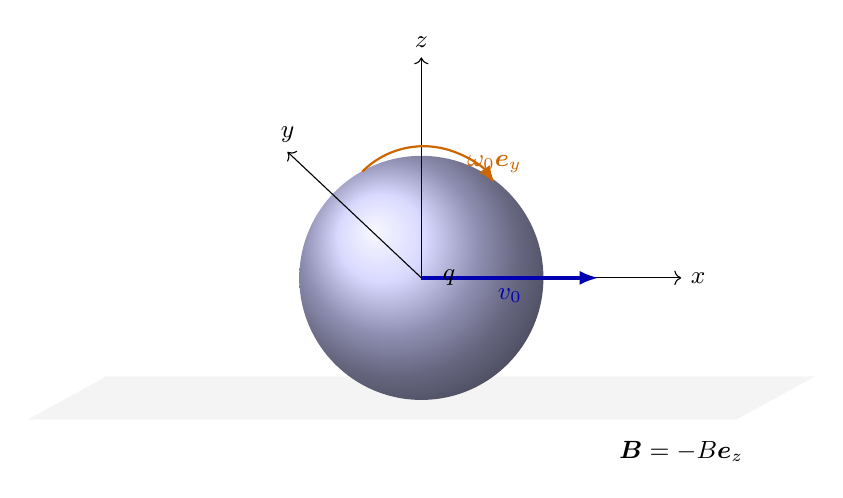
\begin{tikzpicture}[font=\small,x=1cm,y=1cm]
  \fill[gray!9] (-5,-1.25)--(4,-1.25)--(5,-.7)--(-4,-.7)--cycle;
  \shade[ball color=blue!20] (0,.55) circle (1.55);
  \draw[->] (0,.55)--(3.3,.55) node[right] {$x$};
  \draw[->] (0,.55)--(-1.7,2.15) node[above] {$y$};
  \draw[->] (0,.55)--(0,3.35) node[above] {$z$};
  \draw[vec] (0,.55)--(2.25,.55) node[midway,below] {$v_0$};
  \draw[ray] (-.75,1.9) arc (135:35:1.1) node[above] {$\omega_0\bm e_y$};
  \node at (.35,.55) {$q$}; \node at (3.3,-1.65) {$\bm B=-B\bm e_z$};
\end{tikzpicture}

% 10 solution-05
\begin{tikzpicture}[x=1cm,y=1cm,font=\small]

\begin{scope}[shift={(-3.6,0)}]\draw[->](-2.3,0)--(2.6,0)node[right]{$x$};\draw[->](0,-.5)--(0,3.9)node[above]{$y$};\draw[very thick,blue!70](0,1.6)circle(1.6);\draw[guide,green!50!black](0,1.2)circle(1.2);
\fill(0,0)circle(2pt)node[below left]{$C(0)$};\draw[vec](0,0)--(1.3,0)node[below]{$v_0$};\draw[force](0,0)--(0,1.1)node[left]{$F_B$};\draw[force](.25,0)--(.25,-.8)node[right]{$f$};\node[align=center]at(0,-1.7){蓝：中心电荷 $R_c$\\虚线：表面电荷 $R_c'=3R_c/4$};\end{scope}
\begin{scope}[shift={(3.6,1)}]\draw[very thick](0,0)circle(1.5);\draw[very thick,orange!75](0,.75)ellipse(1.299 and .3);\draw[->](0,-1.9)--(0,2)node[above]{$\bm\omega$};\draw[dim](0,.75)--(1.299,.75)node[midway,above]{$r\sin\theta$};\node[align=center]at(0,-2.8){$\mathrm d\mu_m=\mathrm dI\,\pi r^2\sin^2\theta$\\$\bm\mu_m=(qr^2/3)\bm\omega$};\end{scope}
\end{tikzpicture}

% 11 question-06
\begin{tikzpicture}[font=\small,x=1cm,y=1cm]
  \draw[->] (-4.5,0)--(5.2,0) node[right] {$x$};
  \foreach \yy in {-1.4,-.7,0,.7,1.4}{
    \draw[ray] (-4.2,\yy)--(1.0,\yy);
  }
  \draw[very thick,blue!70!black,domain=-2.0:2.0,samples=100,variable=\y]
    plot ({2.6-.42*\y*\y},{\y});
  \draw[very thick,blue!70!black,domain=-2.0:2.0,samples=100,variable=\z]
    plot ({2.6-.42*\z*\z},{.38*\z});
  \foreach \rr in {.55,1.1,1.65,2.0}{
    \pgfmathsetmacro{\xx}{2.6-.42*\rr*\rr}
    \draw[blue!42] (\xx,0) ellipse ({.16*\rr} and \rr);
  }
  \draw[->,blue!55!black] (2.6,0)--(2.6,2.55) node[above] {$y$};
  \draw[->,blue!55!black] (2.6,0)--(3.35,.65) node[right] {$z$};
  \draw[force] (3.5,-2.1)--(2.0,-2.1) node[midway,below] {$v_0$};
  \draw[dim] (0,-2.65)--(2.6,-2.65) node[midway,below] {$l$};
  \node at (-2.3,2.0) {入射平面波 $\omega$};
  \node[align=left,anchor=west] at (3.8,1.2) {$x=l-\alpha(y^2+z^2)-v_0t$\\旋转抛物反射面};
\end{tikzpicture}

% 12 solution-06
\begin{tikzpicture}[x=1cm,y=1cm,font=\small]

\begin{scope}[shift={(-3.7,0)}]\draw[->](-2.6,0)--(2.2,0)node[right]{$x'$};\draw[->](0,-2.6)--(0,2.6)node[above]{$y'$};\draw[very thick,domain=-2.1:2.1,samples=80,variable=\u]plot({1-.4*\u*\u},\u);
\fill(.375,0)circle(2pt)node[below]{$F'$};\foreach\y in{-1.7,1.7}{\draw[ray](-2.4,\y)--({1-.4*\y*\y},\y)--(.375,0);}\node at(0,-3.3){$x_F'=\gamma l-1/(4\gamma\alpha)$};\end{scope}
\begin{scope}[shift={(3.6,0)}]\draw[->](-2,0)--(2.2,0)node[right]{$x$};\draw[->](0,-.5)--(0,3.8)node[above]{$ct$};\draw[very thick,blue!70](1.2,-.3)--(.03,3.6)node[above left]{焦点世界线};
\fill(.96,.5)circle(2pt);\fill(.51,2)circle(2pt);\draw[dim](1.65,.5)--(1.65,2)node[midway,right]{$c\Delta t=\gamma c\Delta t'$};\node[align=center]at(0,-1.6){斜率对应 $\mathrm dx/\mathrm dt=-v_0$\\$\omega_1=\omega'/\gamma=(1+v_0/c)\omega$};\end{scope}
\end{tikzpicture}

% 13 question-07
\begin{tikzpicture}[font=\small,x=1cm,y=1cm]
  \draw[very thick] (-4,-1.6) rectangle (4,1.6);
  \draw[very thick,fill=gray!25] (-2, -1.6) rectangle (-1.82,1.6);
  \node at (-3,0) {$3^\gamma p_0$};
  \node[align=center] at (1.0,.25) {$p_0$\\$T_0$};
  \draw[->] (0,-2.2)--(4.3,-2.2) node[right] {$x$};
  \fill (0,-2.2) circle (2pt) node[below] {$O$};
  \draw[dim] (-4,2.15)--(-2,2.15) node[midway,above] {$1$};
  \draw[dim] (-2,2.15)--(4,2.15) node[midway,above] {$3$};
  \node[right] at (4,0) {绝热气缸};
\end{tikzpicture}

% 14 solution-07
\begin{tikzpicture}[x=1cm,y=1cm,font=\small]

\begin{scope}[shift={(-3.5,0)}]\draw[very thick](-2,-.8)rectangle(2,.8);\draw[guide](-1,-.8)--(-1,.8);\draw[guide](1,-.8)--(1,.8);\draw[->](-2.5,-1.3)--(2.5,-1.3)node[right]{$x/L$};\node[below]at(-1,-1.3){$-.5$};\node[below]at(0,-1.3){$0$};\node[below]at(1,-1.3){$.5$};\draw[vec](-1,1.2)--(1,1.2);\node at(0,1.8){第一次转折点关于中心对称};\node at(0,-2.5){$p_LV_L^\gamma=p_RV_R^\gamma$};\end{scope}
\begin{scope}[shift={(3.7,0)}]\draw[->](-.2,0)--(4.9,0)node[right]{$t$};\draw[->](0,-1.8)--(0,1.8)node[above]{$x/L$};\draw[wave,domain=0:4.6,samples=140]plot(\x,{-1.4*exp(-.25*\x)*cos(260*\x)});\node[align=center]at(2.4,-2.5){振幅慢变示意；$t_2\ll t_3$\\半振幅时转折点 $x/L\simeq\pm.25$};\end{scope}
\end{tikzpicture}

% 15 question-08
\begin{tikzpicture}[font=\small,x=1cm,y=1cm]
  \draw[->] (-4.2,0)--(4.5,0) node[right] {$x,x'$};
  \draw[->] (0,-3.1)--(0,3.4) node[above] {$y$};
  \draw[very thick,blue!70!black] (0,0) circle (2.1);
  \fill (0,0) circle (2pt) node[below left] {$O$};
  \draw[vec] (0,0)--({2.1*cos(38)},{2.1*sin(38)}) node[midway,above] {$R$};
  \draw (1.0,0) arc (0:38:1.0) node[midway,right] {$\theta$};
  \draw[force] (-3.2,-2.6)--(-4.2,-2.6) node[left] {$S':-v\bm e_x$};
  \node at (0,-3.55) {狭义相对论中的转动呼啦圈};
\end{tikzpicture}

% 16 solution-08
\begin{tikzpicture}[x=1cm,y=1cm,font=\small]

\begin{scope}[shift={(-3.5,0)}]\draw[very thick](0,0)circle(1.7);\draw[->](-2.4,0)--(2.6,0)node[right]{$x$};\draw[->](0,-2.1)--(0,3.2)node[above]{$y$};\coordinate(P)at(1.2,1.2);\fill(P)circle(2pt)node[right]{$P$};\fill(0,3)circle(2pt)node[left]{$Q$};\draw[ray](P)--(0,3);\draw[vec](P)--(2,.4)node[right]{$\bm u$};\draw[guide](0,0)--(P);\node[align=center]at(0,-3){顺时针：$\bm u=\omega R(\sin\theta,-\cos\theta)$\\光线从 $P$ 指向 $Q$};\end{scope}
\begin{scope}[shift={(3.5,0)}]\draw[->](-1.4,0)--(2.4,0)node[right]{$x'$};\draw[->](0,-2.7)--(0,2)node[above]{$ct'$};\draw[guide](0,-2.7)--(0,1.7);\fill(0,0)circle(2pt)node[above left]{接收};\fill(1.2,-2)circle(2pt)node[right]{发射};\draw[ray](1.2,-2)--(0,0);\node[align=center]at(.6,-3.6){接收器 $x'=0$ 的世界线竖直\\发射事件 $t'_P<0$\\图为 $x'$ 投影，光线另有 $y'$ 位移};\end{scope}
\end{tikzpicture}

\end{document}
